% --------------------------------------------------------------
% This is all preamble
% --------------------------------------------------------------
 
\documentclass[10pt]{article}


% Basic Packages for Encoding (Input AND Output) and Langauge Support
\usepackage[utf8]{inputenc}
\usepackage[T1]{fontenc}
\usepackage[french]{babel}

% Change Layout with a User-Friendly Interface
\usepackage[margin=1in]{geometry} 

% Include Pictures with a User-Friendly Interface
\usepackage{graphicx}
\graphicspath{ {./images/statistics_and_probability/} }
\usepackage{float}

% Extended Math Support from the Famous 'American Mathematical Society'
\usepackage{amsmath,amsthm,amssymb}

% Section title formatting
\usepackage{titlesec}

\titleformat{\section}
            {\normalfont\scshape}{\thesection}{1em}{}

\newcommand{\N}{\mathbb{N}}
\newcommand{\Z}{\mathbb{Z}}

%Numbered Questions 
\newcounter{question}
\newenvironment{question}
               {\refstepcounter{question}\par\medskip\noindent\textbf{Q~\thequestion.}\par \noindent \rmfamily}
               {\medskip}
 
\begin{document}
 
% --------------------------------------------------------------
%                        Actual content
% --------------------------------------------------------------

\title{Exercices de révision: Statistiques et probabilité}
% \author{Annie B. \thanks{selections from Christos Nikolaidi's original compilation}}
\author{Annie B. \thanks{Les questions sont tirées des examens de l’IB de 2018, 2012, 2011, 2010, 2007}}
\date{\today}
\maketitle

% question template
% \begin{question}
%  \hspace*{\fill} max: 16\par
%  Question material
% \end{question}

\section*{\emph{Calculatrice Graphique Non Permise}}

\begin{question}
  \hspace*{\fill} [Note maximale: 6]\par
  \noindent Un ensemble de données comprend n valeurs.\par
  \noindent La somme des valeurs est de 800 et la moyenne est de 20\par
  \medskip
  
  (a) Trouvez n \hspace*{\fill} [2]\par
  \medskip

  \noindent L’écart type de cet ensemble de données est de 3.\par
  \noindent Chaque valeur de l’ensemble est multipliée par 10.\par
  \medskip  

  (b)\par
     \hspace{1em} (i)  Écrivez la valeur de la nouvelle moyenne. \hspace*{\fill} [2]\par
     \hspace{1em} (ii) Trouvez la valeur de la nouvelle variance.\hspace*{\fill} [2] 
  
\end{question}



\begin{question}
  \hspace*{\fill} [Note maximale: 14]\par
  \noindent Pablo se rend au travail en voiture.\par
  \noindent La probabilité qu’il quitte la maison avant 07 h 00 est de $\frac{3}{4}$.\par
  \noindent S'il quitte la maison avant 07 h 00, la probabilité qu’il soit en retard au travail est de $\frac{1}{8}$.\par 
  \noindent S'il quitte la maison à 07 h 00 ou après, la probabilité qu’il soit en retard au travail est de $\frac{5}{8}$.\par
  \medskip
  (a) Recopiez et complétez le diagramme en arbre suivant.\hspace*{\fill} [3]\par

  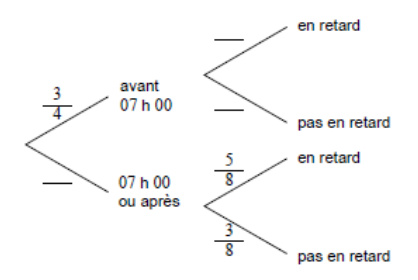
\includegraphics[scale=0.5]{q1_diagram}  

  (b) Trouvez la probabilité que Pablo quitte la maison avant 07 h 00 et qu'il soit en retard.\hspace*{\fill} [2]\par

  (c) Trouvez la probabilité que Pablo soit en retard au travail.\hspace*{\fill} [3]\par

  (d) Sachant que Pablo est en retard au travail,\par
  \hspace{1em}trouvez la probabilité qu’il ait quitté la maison avant 07 h 00.\hspace*{\fill} [3]\par

  (e) Au cours de la semaine prochaine, Pablo se rendra en voiture au travail deux jours.\par
  \hspace{1em}Trouvez la probabilité qu’il soit au moins une fois en retard.\hspace*{\fill} [3]
  
\end{question}


\end{document}
